% Options for packages loaded elsewhere
\PassOptionsToPackage{unicode}{hyperref}
\PassOptionsToPackage{hyphens}{url}
\documentclass[
  12pt,
  oneside]{book}
\usepackage{xcolor}
\usepackage[left=4cm, right=3cm, top=2.5cm, bottom=2.5cm]{geometry}
\usepackage{amsmath,amssymb}
\setcounter{secnumdepth}{5}
\usepackage{iftex}
\ifPDFTeX
  \usepackage[T1]{fontenc}
  \usepackage[utf8]{inputenc}
  \usepackage{textcomp} % provide euro and other symbols
\else % if luatex or xetex
  \usepackage{unicode-math} % this also loads fontspec
  \defaultfontfeatures{Scale=MatchLowercase}
  \defaultfontfeatures[\rmfamily]{Ligatures=TeX,Scale=1}
\fi
\usepackage{lmodern}
\ifPDFTeX\else
  % xetex/luatex font selection
\fi
% Use upquote if available, for straight quotes in verbatim environments
\IfFileExists{upquote.sty}{\usepackage{upquote}}{}
\IfFileExists{microtype.sty}{% use microtype if available
  \usepackage[]{microtype}
  \UseMicrotypeSet[protrusion]{basicmath} % disable protrusion for tt fonts
}{}
\usepackage{setspace}
\makeatletter
\@ifundefined{KOMAClassName}{% if non-KOMA class
  \IfFileExists{parskip.sty}{%
    \usepackage{parskip}
  }{% else
    \setlength{\parindent}{0pt}
    \setlength{\parskip}{6pt plus 2pt minus 1pt}}
}{% if KOMA class
  \KOMAoptions{parskip=half}}
\makeatother
\usepackage{color}
\usepackage{fancyvrb}
\newcommand{\VerbBar}{|}
\newcommand{\VERB}{\Verb[commandchars=\\\{\}]}
\DefineVerbatimEnvironment{Highlighting}{Verbatim}{commandchars=\\\{\}}
% Add ',fontsize=\small' for more characters per line
\usepackage{framed}
\definecolor{shadecolor}{RGB}{248,248,248}
\newenvironment{Shaded}{\begin{snugshade}}{\end{snugshade}}
\newcommand{\AlertTok}[1]{\textcolor[rgb]{0.94,0.16,0.16}{#1}}
\newcommand{\AnnotationTok}[1]{\textcolor[rgb]{0.56,0.35,0.01}{\textbf{\textit{#1}}}}
\newcommand{\AttributeTok}[1]{\textcolor[rgb]{0.13,0.29,0.53}{#1}}
\newcommand{\BaseNTok}[1]{\textcolor[rgb]{0.00,0.00,0.81}{#1}}
\newcommand{\BuiltInTok}[1]{#1}
\newcommand{\CharTok}[1]{\textcolor[rgb]{0.31,0.60,0.02}{#1}}
\newcommand{\CommentTok}[1]{\textcolor[rgb]{0.56,0.35,0.01}{\textit{#1}}}
\newcommand{\CommentVarTok}[1]{\textcolor[rgb]{0.56,0.35,0.01}{\textbf{\textit{#1}}}}
\newcommand{\ConstantTok}[1]{\textcolor[rgb]{0.56,0.35,0.01}{#1}}
\newcommand{\ControlFlowTok}[1]{\textcolor[rgb]{0.13,0.29,0.53}{\textbf{#1}}}
\newcommand{\DataTypeTok}[1]{\textcolor[rgb]{0.13,0.29,0.53}{#1}}
\newcommand{\DecValTok}[1]{\textcolor[rgb]{0.00,0.00,0.81}{#1}}
\newcommand{\DocumentationTok}[1]{\textcolor[rgb]{0.56,0.35,0.01}{\textbf{\textit{#1}}}}
\newcommand{\ErrorTok}[1]{\textcolor[rgb]{0.64,0.00,0.00}{\textbf{#1}}}
\newcommand{\ExtensionTok}[1]{#1}
\newcommand{\FloatTok}[1]{\textcolor[rgb]{0.00,0.00,0.81}{#1}}
\newcommand{\FunctionTok}[1]{\textcolor[rgb]{0.13,0.29,0.53}{\textbf{#1}}}
\newcommand{\ImportTok}[1]{#1}
\newcommand{\InformationTok}[1]{\textcolor[rgb]{0.56,0.35,0.01}{\textbf{\textit{#1}}}}
\newcommand{\KeywordTok}[1]{\textcolor[rgb]{0.13,0.29,0.53}{\textbf{#1}}}
\newcommand{\NormalTok}[1]{#1}
\newcommand{\OperatorTok}[1]{\textcolor[rgb]{0.81,0.36,0.00}{\textbf{#1}}}
\newcommand{\OtherTok}[1]{\textcolor[rgb]{0.56,0.35,0.01}{#1}}
\newcommand{\PreprocessorTok}[1]{\textcolor[rgb]{0.56,0.35,0.01}{\textit{#1}}}
\newcommand{\RegionMarkerTok}[1]{#1}
\newcommand{\SpecialCharTok}[1]{\textcolor[rgb]{0.81,0.36,0.00}{\textbf{#1}}}
\newcommand{\SpecialStringTok}[1]{\textcolor[rgb]{0.31,0.60,0.02}{#1}}
\newcommand{\StringTok}[1]{\textcolor[rgb]{0.31,0.60,0.02}{#1}}
\newcommand{\VariableTok}[1]{\textcolor[rgb]{0.00,0.00,0.00}{#1}}
\newcommand{\VerbatimStringTok}[1]{\textcolor[rgb]{0.31,0.60,0.02}{#1}}
\newcommand{\WarningTok}[1]{\textcolor[rgb]{0.56,0.35,0.01}{\textbf{\textit{#1}}}}
\usepackage{longtable,booktabs,array}
\usepackage{calc} % for calculating minipage widths
% Correct order of tables after \paragraph or \subparagraph
\usepackage{etoolbox}
\makeatletter
\patchcmd\longtable{\par}{\if@noskipsec\mbox{}\fi\par}{}{}
\makeatother
% Allow footnotes in longtable head/foot
\IfFileExists{footnotehyper.sty}{\usepackage{footnotehyper}}{\usepackage{footnote}}
\makesavenoteenv{longtable}
\usepackage{graphicx}
\makeatletter
\newsavebox\pandoc@box
\newcommand*\pandocbounded[1]{% scales image to fit in text height/width
  \sbox\pandoc@box{#1}%
  \Gscale@div\@tempa{\textheight}{\dimexpr\ht\pandoc@box+\dp\pandoc@box\relax}%
  \Gscale@div\@tempb{\linewidth}{\wd\pandoc@box}%
  \ifdim\@tempb\p@<\@tempa\p@\let\@tempa\@tempb\fi% select the smaller of both
  \ifdim\@tempa\p@<\p@\scalebox{\@tempa}{\usebox\pandoc@box}%
  \else\usebox{\pandoc@box}%
  \fi%
}
% Set default figure placement to htbp
\def\fps@figure{htbp}
\makeatother
\setlength{\emergencystretch}{3em} % prevent overfull lines
\providecommand{\tightlist}{%
  \setlength{\itemsep}{0pt}\setlength{\parskip}{0pt}}
\usepackage[style=apa,]{biblatex}
\addbibresource{book.bib}
\addbibresource{packages.bib}
\addbibresource{test.bib}
\usepackage[none]{hyphenat}
\pagestyle{plain}
\raggedbottom
\usepackage[nottoc,notlot,notlof]{tocbibind}
\usepackage{pdfpages}
\usepackage[width=\textwidth]{caption}

\usepackage{fancyhdr}
\pagestyle{fancy}
\fancyhf{}
\setlength{\headheight}{15pt}%
\fancyhead[RO,RE]{\nouppercase{\leftmark}}
\fancyfoot[CO, CE] {\thepage}
\renewcommand{\headrulewidth}{0pt}
\renewcommand{\footrulewidth}{0pt}
\usepackage{booktabs}
\usepackage{longtable}
\usepackage{array}
\usepackage{multirow}
\usepackage{wrapfig}
\usepackage{float}
\usepackage{colortbl}
\usepackage{pdflscape}
\usepackage{tabu}
\usepackage{threeparttable}
\usepackage{threeparttablex}
\usepackage[normalem]{ulem}
\usepackage{makecell}
\usepackage{xcolor}
\usepackage{bookmark}
\IfFileExists{xurl.sty}{\usepackage{xurl}}{} % add URL line breaks if available
\urlstyle{same}
\hypersetup{
  pdftitle={CASA dissertation using Bookdown},
  hidelinks,
  pdfcreator={LaTeX via pandoc}}

\title{CASA dissertation using Bookdown}
\author{Yifan Wu\\
\strut \\
CASA0010, MSc Smart Cities Dissertation\\
\strut \\
Supervisor: Dr Andrew MacLachlan\\
\strut \\
Repository: \url{https://andrewmaclachlan.github.io/CASA0005repo/}\\
\strut \\
This dissertation is submitted in part requirement for the\\
MSc (Or MRes) in the Centre for Advanced Spatial Analysis,\\
Bartlett Faculty of the Built Environment, UCL\\
\strut \\
Word count:}
\date{2025-06-26}

\begin{document}
\maketitle

\setstretch{1.5}
\pagenumbering{roman}

\chapter*{Abstract}\label{abstract}

Some abstract text

\pagenumbering{roman}

\chapter*{Declaration}\label{declaration}

I hereby declare that this dissertation is all my own original work and that all sources have been acknowledged. It is xxx words in length

\chapter*{Acknowledgements}\label{acknowledgements}

I would like to thank blah blah

% Trigger ToC creation in LaTeX
\setcounter{tocdepth}{3}
\tableofcontents
\listoffigures
\listoftables

\chapter*{Abbreviations}\label{abbreviations}

\begin{table}
\centering
\begin{tabular}{ll}
\toprule
\textbf{Term} & \textbf{Abbreviation}\\
\midrule
Digital Elevation Model & DEM\\
Digital Surface Model & DSM\\
Digital Terrain Model & DTM\\
\bottomrule
\end{tabular}
\end{table}

\chapter{Bookdown basics}\label{bookdown-basics}

\pagenumbering{arabic} 

Bookdown enables us to take raw text files (e.g.~Rmarkdown files) and output them into a number of different formats with ease. This is more useful than LaTex as you can create a word version for comments from your supervisor, a pdf for final submission and an online book for your own portfolio.

\section{Structure}\label{structure}

A bookdown book simply combines multiple Rmarkdown files into .pdf, html or .epub (but i've disabled epub here).

All Rmakdown files must be located in the base (or root) of the project. For example, don't got putting the .Rmd in a folder called chapters and then wonder why it's not working. They all must be in the same folder as the project file. You can however put output figure images into a folder (e.g.~figures) then call them in.

\section{Building the book}\label{building-the-book}

You will need the packages: \texttt{bookdown,\ kabble,\ knitr}

You also need to install \texttt{tinytex::install\_tinytex()} for generating .pdfs from your book.

Once installed you can build the book by clicking the Build Book icon under the build tab in the top right quadrant.

To export the book to word follow the code below from \href{https://www.eddjberry.com/post/writing-your-thesis-with-bookdown/}{Edd Berry}:

\begin{Shaded}
\begin{Highlighting}[]
\NormalTok{bookdown}\SpecialCharTok{::}\FunctionTok{preview\_chapter}\NormalTok{(}\StringTok{"01{-}intro.Rmd"}\NormalTok{,}
                \AttributeTok{output\_format =} \StringTok{"bookdown::word\_document2"}\NormalTok{,}
                \AttributeTok{output\_file =} \FunctionTok{paste0}\NormalTok{(}\StringTok{"thesis{-}intro{-}"}\NormalTok{, }
                                     \FunctionTok{format}\NormalTok{(}\FunctionTok{Sys.Date}\NormalTok{(), }
\NormalTok{                                            (}\StringTok{"\%d{-}\%m{-}\%y"}\NormalTok{)), }
                                     \StringTok{".docx"}\NormalTok{),}
                \AttributeTok{output\_dir =} \StringTok{"chapter{-}previews"}\NormalTok{)}
\end{Highlighting}
\end{Shaded}

You can also setup a reference document if you wish that word will style it on. To do so:

\begin{enumerate}
\def\labelenumi{\arabic{enumi}.}
\tightlist
\item
  export to word using the code above.
\item
  change the headings styles in word
\item
  save the document
\item
  add the \texttt{output\_options()} function to the code above
\end{enumerate}

See \href{https://bookdown.org/yihui/rmarkdown-cookbook/word-template.html}{Custom Word Templates} for more detailed instructions.

\begin{Shaded}
\begin{Highlighting}[]
\NormalTok{bookdown}\SpecialCharTok{::}\FunctionTok{preview\_chapter}\NormalTok{(}\StringTok{"01{-}intro.Rmd"}\NormalTok{,}
                \AttributeTok{output\_format =} \StringTok{"bookdown::word\_document2"}\NormalTok{,}
                \AttributeTok{output\_file =} \FunctionTok{paste0}\NormalTok{(}\StringTok{"thesis{-}intro{-}"}\NormalTok{, }
                                     \FunctionTok{format}\NormalTok{(}\FunctionTok{Sys.Date}\NormalTok{(), }
\NormalTok{                                            (}\StringTok{"\%d{-}\%m{-}\%y"}\NormalTok{)), }
                                     \StringTok{".docx"}\NormalTok{),}
                \AttributeTok{output\_dir =} \StringTok{"chapter{-}previews"}\NormalTok{,}
                \AttributeTok{output\_options =} \FunctionTok{list}\NormalTok{(}\AttributeTok{reference\_docx =} \StringTok{"word{-}style{-}ref.docx"}\NormalTok{))}
\end{Highlighting}
\end{Shaded}

You can also export the whole document as word by clicking Build Book and selecting it. However, note that tables built with \texttt{Kabble} don't work with word, so you have the following options

\begin{itemize}
\tightlist
\item
  create the html (gitbook) and copy the tables into word
\item
  either exclude them (\texttt{eval=FALSE}) in the code chunk header
\item
  use .pdf.
\end{itemize}

\section{YAMLs}\label{yamls}

You will see some files with a \texttt{.yml} extension. These stand for yet another markup language.

Open the \texttt{\_output.yml} and \texttt{\_bookdown.yml}.

The \texttt{\_output.yml} controls the settings for each outputted format.

The \texttt{\_bookdown.yml} controls the order in which the files are made into chapters - you can also change the \texttt{Chapter} title if you wish here.

I have set these up to create nice outputs, so there is really no need to change anything, unless you want to add a new chapter and include it in the list. To do so, simply create a new Rmarkdown document, delete all the default content, add a first level heading, and the then add it to where you want it to appear in the document in the \texttt{\_bookdown.yml}.

\section{Formatting}\label{formatting}

You'll notice in the \texttt{\_output.yml} that the various formats (html (or gitbook) and pdf) are calling styling codes. The gitbook calls \texttt{style.css} and the \texttt{pdf\_book} calls \texttt{preamble.tex}. These files just style the various outputs.

I have copied in a basic styling with a CASA logo in the table of contents, you can replace this with other variations of the file if you wish or look at the \href{https://github.com/rstudio/bookdown-demo}{minimal bookdown example} or my \href{https://github.com/andrewmaclachlan/CASA0005repo/blob/master/assets/style.css}{CASA0005 .css file}.

The best place to learn more about styling is the \href{https://rstudio4edu.github.io/rstudio4edu-book/intro-bookdown.html}{RStudio for education bookdown guide}

For the .pdf version in the \texttt{preamble.tex} we have to use LaTex code. I am by no means an expert in this. If you Google each package it will tell you what it does. There isn't much here really, but all the header stuff refers to the headings at the top of each page.

This tutorial from OurCoding Club explains some of the LaTex packages in a bit more detail: \url{https://ourcodingclub.github.io/tutorials/rmarkdown-dissertation/}

\section{Index file}\label{index-file}

Open up the \texttt{index.Rmd} this \texttt{Rmd} must be called first in the \texttt{\_bookdown.yml} list. There are a number of options here, but i've set them all up to be compliant with the CASA thesis requirements.

You will need to change your title and name etc. Make sure you leave the a space here: \texttt{\textbar{}\ Andrew\ MacLachlan} this won't work \texttt{\textbar{}Andrew\ MacLachlan}

If you were to be printing your work, you'd want to change the \texttt{classoption} to \texttt{twosides} and make sure the \texttt{geometry\ margins} were correct. \texttt{linestrech} refers to the line spacing and the bibliography stuff we come on to later.

Input your GitHub repo and add a description.

If you ever wanted to just create a report and not a thesis you can change the \texttt{documentclass} to other options such \texttt{report}, \texttt{article} or \texttt{letter}

\section{Preamble}\label{preamble}

Open the \texttt{preable.Rmd} and you will see all the sections that are required before the main text (e.g.~Declaration and so on). At the top of the page i've used a code chunk set to LaTex, saying to use Roman numbering as we don't want page 1 to be the Declaration, we want it to be the first page of the Introduction. There are two conditions for each of the sections that state if output to HTML (gitbook) then do this, if output to LaTex then do this. This is the only place we have this. In our bookdown HTML we want to be able to click these sections, but in our LaTex .pdf we don't want them to appear in the table of contents. This is what this code is doing.

The Abstract is on the \texttt{index.Rmd} the same code condition applies to it, with Roman numbering also specified.

If you look back in the \texttt{\_output.yml} you'll also see the \texttt{toc} (table of contents) is set to false. By default this appears right after the title, but we want this to come after our \texttt{preable.Rmd}. You'll see that i've called \texttt{\textbackslash{}tableofcontents}, \texttt{\textbackslash{}listoffigures} and \texttt{\textbackslash{}listoftables} in the correct place again using a LaTex code chunk. These aren't required for the bookdown output.

The last section here is the abbreviations. To make this really easy, i've created an excel document to add them into. The code here will load that and then use the \texttt{kable} package to make a table. More on this later.I've also done the same for the research log in the appendix --- excel sheet called \texttt{research\_log}.

\section{Change this to a thesis}\label{change-this-to-a-thesis}

Easy. Just change all the titles to what you want (e.g.~Introduction, Literature Review, Methodology, Discussion, Conclusion). Some of the latter \texttt{.Rmds} (Discussion etc) are ready to go!

\section{Word count}\label{word-count}

To get a word count install and then use the \href{https://github.com/benmarwick/wordcountaddin}{word count addin package} through Tools\textgreater Addins\textgreater Wordcount

\section{Adding a pdf}\label{adding-a-pdf}

If you wish to add another .pdf as an Appendix (in your .pdf) then again we need a bit of LaTex code

\texttt{\textbackslash{}includepdf{[}pages=\{-\}{]}\{mypdf.pdf\}}

If you look in the \texttt{08-Appendix.Rmd} then you will see another if LaTex section, simply add in the line of code above, replacing \texttt{mypdf.pdf} with your pdf title in the main project folder. It will then be appended to the thesis. Of course, this isn't required in the online book, but you just link to them on GitHub or embed .pdfs using:

You'd need a condition around this like in the \texttt{preamble.Rmd} but a link is fine. I embedded a .pdf in \href{https://andrewmaclachlan.github.io/CASA0005repo/assignment-resources-1.html}{the assignment resources of CASA0005}

\section{Writing code}\label{writing-code}

Use one project for your thesis and another for your analysis. Don't try and do it all in a thesis project. You can set your output folder from your main analysis project to the thesis project and then easily load the figures in.

\section{Package reproducibility}\label{package-reproducibility}

Have you ever created an R script, come back to it 6 months later and wonder why it's not working correctly? It's probably because of package updates.

\texttt{renv} (pronounced R - env) can capture the packages used in your project and re-create your current library. You simply:

\begin{enumerate}
\def\labelenumi{\arabic{enumi}.}
\tightlist
\item
  Create a new project - \texttt{renv::init()}
\item
  Create a snapshot - \texttt{renv::snapshot()}
\item
  Call the snapshot to load - \texttt{renv::restore()}
\end{enumerate}

The package information and dependencies are stored in a \texttt{renv.lock} file.

When R loads a package it gets it from the library path, which is where the packages live. Sometimes there are two libraries a system and a user library - use \texttt{.libPaths()}. The system library = the packages with R, the user library = packages you have installed.

When you load a package it loads the first instance it comes across, user comes before system. To check - \texttt{find.package("tidyverse")}

All your projects use these paths! If you load different packages and versions of them + dependencies. E.g.

\begin{itemize}
\tightlist
\item
  Project 1 used \texttt{sf} version 0.9-8
\item
  Project 2 used \texttt{sf} version 0.9-6
\end{itemize}

Switching between projects would mean you have the wrong version as they use the same libraries.

\texttt{renv} - each project gets it's own library! Project local libraries.

When you use \texttt{renv::init()} the library path will be changed to a project local one.

It will create a lock file that holds all the package information.

To re-create my environment once you have forked and pulled this repository you would use \texttt{renv::restore()}.

Of coruse some projects use the same package version --- such as \texttt{tidyverse}, \texttt{renv} has a global cache of all the libraries. So there is a massive database of your libraries then each project library links it from there, meaning you don't have 10 versions of the same \texttt{tidyverse}.

You can also interact with \texttt{git}

\begin{itemize}
\tightlist
\item
  \texttt{renv::history()} --- finds the commits where the lock file changed
\item
  \texttt{renv::revert(commit\ =\ "id")} --- changes the lock file back to what it was at a commit
\end{itemize}

For more information watch renv: Project Environments for R introduction video: \url{https://www.rstudio.com/resources/rstudioconf-2020/renv-project-environments-for-r/}

\chapter{Cross referencing}\label{crossref}

\section{Chapters or sections}\label{chapters-or-sections}

Always give you sections an additional reference\ldots e.g.~\texttt{\#\ Cross\ referencing\ \{\#crossref\}} This gives us two reference points. The first we can use to reference the section name\ldots{}

\begin{enumerate}
\def\labelenumi{\arabic{enumi}.}
\tightlist
\item
  We want to say see the Introduction (or other section label)we use \ldots{}\texttt{{[}Cross\ referencing{]}} giving \hyperref[crossref]{Cross referencing}
\end{enumerate}

But what if we want to reference the section number (e.g.~Chapter 1 or section 4.2)

\begin{enumerate}
\def\labelenumi{\arabic{enumi}.}
\tightlist
\item
  Just reference the label we gave to the section\ldots.see Chapter \texttt{\textbackslash{}@ref(crossref)} giving see Chapter \ref{crossref}
\end{enumerate}

\section{Figures, tables, even code chunks}\label{figures-tables-even-code-chunks}

\subsection{Figures}\label{figures}

When you create a figure, table or code chunk there is an option to name the chunk something. Do it!. Don't be like me and not! Be warned that these chunk names can't have any fancy or strange characters in them e.g.~\_. I think a - is allowed, but i'd keep it simple. Here is a figure. In the chunk options after \texttt{r} i have specified \texttt{nice-fig,\ echo=FALSE,\ fig.cap=\textquotesingle{}Here\ is\ a\ nice\ figure!\textquotesingle{},\ out.width=\textquotesingle{}80\%\textquotesingle{}}

\begin{figure}
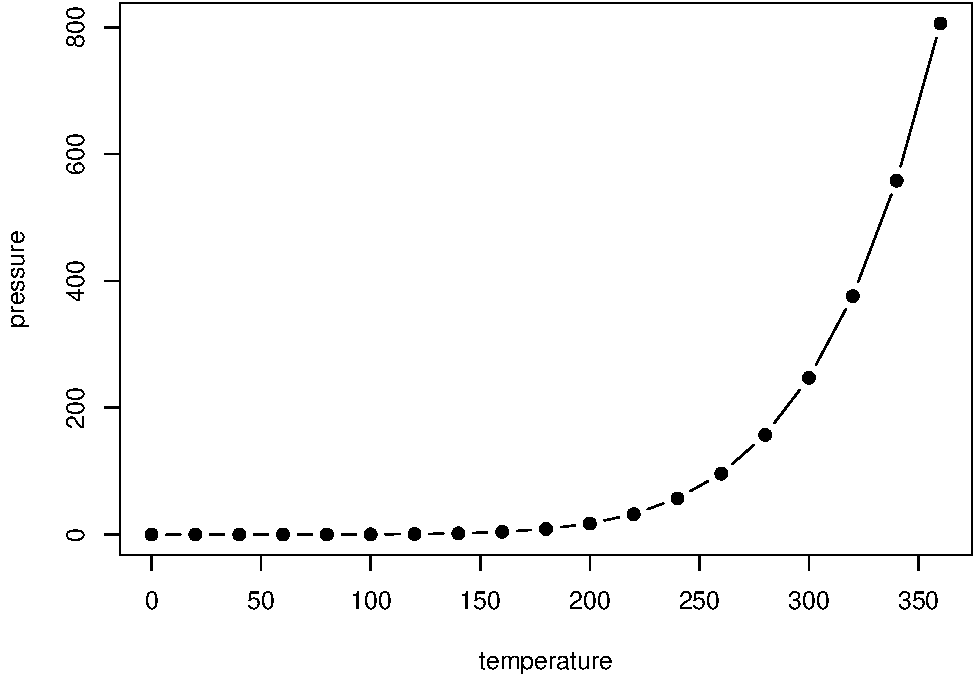
\includegraphics[width=0.8\linewidth]{CASA-Thesis_files/figure-latex/nice-fig-1} \caption{Here is a nice figure!}\label{fig:nice-fig}
\end{figure}

To cross reference this just include Figure \texttt{\textbackslash{}@ref(fig:nice-fig)} which gives\ldots Figure \ref{fig:nice-fig}.

\subsection{Tables}\label{tables}

For tables i'd recommend using the \texttt{kable} package. Here is an example table, same deal as the \hyperref[figures]{Figures} section with naming the code chunk.

\begin{Shaded}
\begin{Highlighting}[]
\NormalTok{knitr}\SpecialCharTok{::}\FunctionTok{kable}\NormalTok{(}
  \FunctionTok{head}\NormalTok{(iris, }\DecValTok{20}\NormalTok{), }\AttributeTok{caption =} \StringTok{\textquotesingle{}Here is a nice table!\textquotesingle{}}\NormalTok{,}
  \AttributeTok{booktabs =} \ConstantTok{TRUE}
\NormalTok{)}
\end{Highlighting}
\end{Shaded}

\begin{table}

\caption{\label{tab:nice-tab}Here is a nice table!}
\centering
\begin{tabular}[t]{rrrrl}
\toprule
Sepal.Length & Sepal.Width & Petal.Length & Petal.Width & Species\\
\midrule
5.1 & 3.5 & 1.4 & 0.2 & setosa\\
4.9 & 3.0 & 1.4 & 0.2 & setosa\\
4.7 & 3.2 & 1.3 & 0.2 & setosa\\
4.6 & 3.1 & 1.5 & 0.2 & setosa\\
5.0 & 3.6 & 1.4 & 0.2 & setosa\\
\addlinespace
5.4 & 3.9 & 1.7 & 0.4 & setosa\\
4.6 & 3.4 & 1.4 & 0.3 & setosa\\
5.0 & 3.4 & 1.5 & 0.2 & setosa\\
4.4 & 2.9 & 1.4 & 0.2 & setosa\\
4.9 & 3.1 & 1.5 & 0.1 & setosa\\
\addlinespace
5.4 & 3.7 & 1.5 & 0.2 & setosa\\
4.8 & 3.4 & 1.6 & 0.2 & setosa\\
4.8 & 3.0 & 1.4 & 0.1 & setosa\\
4.3 & 3.0 & 1.1 & 0.1 & setosa\\
5.8 & 4.0 & 1.2 & 0.2 & setosa\\
\addlinespace
5.7 & 4.4 & 1.5 & 0.4 & setosa\\
5.4 & 3.9 & 1.3 & 0.4 & setosa\\
5.1 & 3.5 & 1.4 & 0.3 & setosa\\
5.7 & 3.8 & 1.7 & 0.3 & setosa\\
5.1 & 3.8 & 1.5 & 0.3 & setosa\\
\bottomrule
\end{tabular}
\end{table}

Now to cite the table it's just Table \texttt{\textbackslash{}@ref(tab:nice-tab)}, giving Table \ref{tab:nice-tab}

\section{Citing documents}\label{citing-documents}

To cite documents they need to be in a \texttt{.bib} file, that must be loaded within your \texttt{index.Rmd} with the \texttt{bibliography:} argument. Have a look at my \texttt{index.Rmd} and you will see there are three such files, two that were provided as an example here \texttt{book.bib}, \texttt{packages.bib} and one that i added \texttt{test.bib}. I can simply cite the papers within them using the citation key e.g.~\texttt{{[}@xie2015{]}} giving \autocite{xie2015}. Make sure you remove the ones you don't need.

If you remove the citation from the \texttt{{[}{]}} it will give \textcite{xie2015}.

When citing multiple authors use a ; \texttt{{[}@xie2015;\ @maclachlan2017urban{]}} = \autocite{xie2015,maclachlan2017urban}

To remove the author add a minus sign \texttt{-@maclachlan2017urban} = \autocite*{maclachlan2017urban}

\section{Citing using software}\label{citing-using-software}

Zotero can now continuously update your \texttt{.bib} file.

To do so:

\begin{enumerate}
\def\labelenumi{\arabic{enumi}.}
\item
  Download the latest release --- the \texttt{.xpi} file: \url{https://github.com/retorquere/zotero-better-bibtex/releases/tag/v5.2.108}
\item
  In Zotero \textgreater{} Tools \textgreater{} Add ons \textgreater{} Extensions
\item
  Select the cog \textgreater{} Install add on from file
\item
  Select the \texttt{.xip} \textgreater{} restart Zotero.
\end{enumerate}

On the restart select the default naming convention.

To export the library

\begin{enumerate}
\def\labelenumi{\arabic{enumi}.}
\item
  File \textgreater{} export
\item
  Select Better BibLaTex
\item
  Click keep updated
\item
  Select the file to save into your Thesis project
\item
  Make sure you have the file listed in your \texttt{bibliography} in the \texttt{index.Rmd} file
\end{enumerate}

You can also manage references using \texttt{citr} which makes finding them to cite much easier. In RStudio go: Addins (top tool bar) \textgreater{} insert citations.

\section{Footnotes}\label{footnotes}

To add a footnote use \texttt{\^{}{[}This\ is\ a\ footnote{]}} to create \footnote{This is a footnote}.

\chapter{Equations and direct quotes}\label{equations-and-direct-quotes}

This section will focus on equations and direct quotes

\section{Equations}\label{equations}

You need to include equations with some LaTeX. The easiest way to do this is to use an online tool such as: \url{https://latex.codecogs.com/eqneditor/editor.php}. It can be a real pain to get these right, but once you've worked it out it will be much easier than dealing with word equation editor.

\begin{equation} 
  p= h\frac{c}{\varrho}
  \label{eq:test}
\end{equation}

To reference this in the text we use: \eqref{eq:test}

You can also test your code in your RMarkdown document using \texttt{\$} e.g.~\[p= h\frac{c}{\varrho}\]

However, this won't generate an equation number and you can't cross reference it. But we can use this logic to define the parameters within the equation e.g.~where \(h\) is Plank's constant, \(6.626 × 10^-34 Js\)

\texttt{\$\$} puts it on a new line, single \texttt{\$} keeps it on the same line (in the text)

\section{Block quotes (or direct quotes)}\label{quotes}

You may wish to quote a large section from a source, to do this use a block quote.

Simply input a \texttt{\textgreater{}} before the text. For example \texttt{\textgreater{}\ This\ is\ a\ quote}.

\begin{quote}
``This is a direct quote''
\end{quote}

You can also provide an attribution at the footer of the quote using \texttt{tufte::quote\_footer()}, either a name or a reference. You'll need to install the \texttt{tufte} package to use this. For example, \texttt{\textgreater{}\ {[}include\ only\ r\ here{]}\ tufte::quote\_footer(\textquotesingle{}-\/-\/-\ Joe\ Martin\textquotesingle{})} or \texttt{\textgreater{}\ {[}include\ only\ r\ here{]}\ tufte::quote\_footer(\textquotesingle{}-\/-\/-\ @xie2015\textquotesingle{})}

Giving\ldots{}

\begin{quote}
\hfill --- Joe Martin
\end{quote}

\begin{quote}
\hfill --- \textcite{xie2015}
\end{quote}

Instead you could just include the reference at the end of the quote, using the same method to reference as we've seen before..e.g. \texttt{\textgreater{}\ "This\ is\ a\ direct\ quote"\ @xie2015,\ Equation\ \textbackslash{}@ref(eq:test)}\ldots giving

\begin{quote}
``This is a direct quote'' \textcite{xie2015} \eqref{eq:test}
\end{quote}

\chapter{Figures, tables, hosting GitBook}\label{figures-tables-hosting-gitbook}

This section is going to focus including figures and creating tables

\begin{figure}
\includegraphics[width=300pt]{general_images/example_flow} \caption{Summary of methdological procedure for (a).... and (b)....}\label{fig:methodsflow}
\end{figure}

\section{Including figures and tables}\label{including-figures-and-tables}

\subsection{Figures}\label{figures-1}

To include the figure above use the code:

\texttt{knitr::include\_graphics(here::here(\textquotesingle{}general\_images\textquotesingle{},\textquotesingle{}example\_flow.png\textquotesingle{}))}

within a code chunk. In the chunk options you can specify the width and figure captions e.g.~

\texttt{out.width="100pt",\ fig.cap="Summary\ of\ methdological\ procedure\ for\ (a)....\ and\ (b)...."}.

However, if you do show the code with \texttt{echo=TRUE} then you can't specify the \texttt{out.width}.

For making flow diagrams have a look at:

\begin{enumerate}
\def\labelenumi{\arabic{enumi}.}
\tightlist
\item
  Lucidchart
\item
  Draw.io
\end{enumerate}

\subsection{Tables}\label{tables-1}

For creating tables i'd suggest creating either an excel file or \texttt{.csv} and then reading the data into R and using the \texttt{kabble} package to format it how you wish. The example below is from the abbreviations section

\begin{Shaded}
\begin{Highlighting}[]
\FunctionTok{library}\NormalTok{(tidyverse)}
\FunctionTok{library}\NormalTok{(knitr)}
\FunctionTok{library}\NormalTok{(kableExtra)}
\FunctionTok{library}\NormalTok{(readxl)}
\FunctionTok{library}\NormalTok{(fs)}
\FunctionTok{library}\NormalTok{(here)}

\CommentTok{\#read in data}
\FunctionTok{read\_excel}\NormalTok{(}\FunctionTok{here}\NormalTok{(}\StringTok{"tables"}\NormalTok{, }\StringTok{"abbreviations.xlsx"}\NormalTok{))}\SpecialCharTok{\%\textgreater{}\%}
  \FunctionTok{arrange}\NormalTok{(Term) }\SpecialCharTok{\%\textgreater{}\%} \CommentTok{\# i.e. alphabetical order by Term}
  \CommentTok{\# booktab = T gives us a pretty APA{-}ish table}
\NormalTok{  knitr}\SpecialCharTok{::}\FunctionTok{kable}\NormalTok{(}\AttributeTok{booktabs =} \ConstantTok{TRUE}\NormalTok{)}\SpecialCharTok{\%\textgreater{}\%} 
  \FunctionTok{kable\_styling}\NormalTok{(}\AttributeTok{position =} \StringTok{"center"}\NormalTok{)}\SpecialCharTok{\%\textgreater{}\%}
  \CommentTok{\# any specifc row changes you want}
    \FunctionTok{row\_spec}\NormalTok{(.,}
  \AttributeTok{row=}\DecValTok{0}\NormalTok{,}
  \AttributeTok{bold =} \ConstantTok{TRUE}\NormalTok{)}
\end{Highlighting}
\end{Shaded}

\begin{table}
\centering
\begin{tabular}{ll}
\toprule
\textbf{Term} & \textbf{Abbreviation}\\
\midrule
Digital Elevation Model & DEM\\
Digital Surface Model & DSM\\
Digital Terrain Model & DTM\\
\bottomrule
\end{tabular}
\end{table}

You do loads of things with kabble including adding small visulisations within the table - \href{https://cran.r-project.org/web/packages/kableExtra/vignettes/awesome_table_in_html.html\#Overview}{consult the documentation for more info}.

\textbf{If in doubt, keep it simple}

other useful arguments for tables:

\begin{itemize}
\item
  \texttt{column\_spec(2,\ width\ =\ "9cm")} = set column width
\item
  \texttt{kable(timeline,longtable\ =\ T....}= allow the table to go over multiple pages
\end{itemize}

For example\ldots{}
\newpage

\begin{Shaded}
\begin{Highlighting}[]
\FunctionTok{read\_excel}\NormalTok{(}\FunctionTok{here}\NormalTok{(}\StringTok{"tables"}\NormalTok{, }\StringTok{"policy.xlsx"}\NormalTok{))}\SpecialCharTok{\%\textgreater{}\%}
  \FunctionTok{mutate\_all}\NormalTok{(}\SpecialCharTok{\textasciitilde{}} \FunctionTok{replace\_na}\NormalTok{(.x, }\StringTok{""}\NormalTok{)) }\SpecialCharTok{\%\textgreater{}\%}
  \CommentTok{\# booktab = T gives us a pretty APA{-}ish table}
\NormalTok{  knitr}\SpecialCharTok{::}\FunctionTok{kable}\NormalTok{(}\AttributeTok{longtable =}\NormalTok{ T, }\AttributeTok{booktabs =}\NormalTok{ T, }
               \AttributeTok{caption =} \StringTok{\textquotesingle{}Relevant influential international, metropolitan and local UHI and urban expansion policies, strategies and assessments (with publication date) referred to in this paper. * Denotes documents that lack specific UHI related policy but recognise the value of maintaining vegetation.\textquotesingle{}}\NormalTok{)}\SpecialCharTok{\%\textgreater{}\%} 
  \FunctionTok{kable\_styling}\NormalTok{(}\AttributeTok{position =} \StringTok{"center"}\NormalTok{, }\AttributeTok{full\_width =}\NormalTok{ T)}\SpecialCharTok{\%\textgreater{}\%}
  \CommentTok{\# any specifc row changes you want}
    \FunctionTok{row\_spec}\NormalTok{(.,}
  \AttributeTok{row=}\FunctionTok{c}\NormalTok{(}\DecValTok{0}\NormalTok{,}\DecValTok{1}\NormalTok{,}\DecValTok{8}\NormalTok{, }\DecValTok{18}\NormalTok{),}
  \AttributeTok{bold =} \ConstantTok{TRUE}\NormalTok{)}\SpecialCharTok{\%\textgreater{}\%}
  \FunctionTok{column\_spec}\NormalTok{(}\DecValTok{1}\NormalTok{, }\AttributeTok{width =} \StringTok{"14cm"}\NormalTok{)}\SpecialCharTok{\%\textgreater{}\%}
  \FunctionTok{row\_spec}\NormalTok{(}\FunctionTok{c}\NormalTok{(}\DecValTok{1}\NormalTok{, }\DecValTok{8}\NormalTok{, }\DecValTok{18}\NormalTok{), }\AttributeTok{hline\_after =}\NormalTok{ T)}
\end{Highlighting}
\end{Shaded}

\begin{longtabu} to \linewidth {>{\raggedright\arraybackslash}p{14cm}}
\caption{\label{tab:kable}Relevant influential international, metropolitan and local UHI and urban expansion policies, strategies and assessments (with publication date) referred to in this paper. * Denotes documents that lack specific UHI related policy but recognise the value of maintaining vegetation.}\\
\toprule
\textbf{Policy}\\
\midrule
\textbf{International}\\
\midrule
United Nations The World Cities in 2016 (2016)\\
United Nations New Urban Agenda (2017)\\
ARUP City Resilience Framework (2015)\\
United Nations International Strategy for Disaster Reduction Sendai Framework (2015)\\
\addlinespace
Universal Sustainable Development Goals (2015)\\
Biological Diversity, Cities and Biodiversity Outlook (2012)\\
\textbf{Metropolitan}\\
\midrule
AECOM Australia, Economic Assessment of the Urban Heat Island Effect, Melbourne (2012)\\
The Spatial Development Strategy For Greater London (2017)\\
\addlinespace
Western Australia Planning Commission, Perth and Peel @3.5 million (2015)\\
City of Johannesburg Metropolitan Municipality, Spatial Development Framework 2040 (2016)\\
Western Australian Planning Commission, Directions 2031 and beyond: metropolitan planning beyond the horizon (2010)\\
Western Australian Planning Commission, Development Control Policy 2.3 Public Open Space in Residential Areas (2002)\\
Plan For The Metropolitan Region Perth And Fremantle (1955)\\
\addlinespace
Singapore Government, Open Space Provision (2011)\\
Western Australian Planning Commission, Metropolitan Region Scheme Text (2006)\\
\textbf{Local}\\
\midrule
USA Environmental Protection Agency, Reducing Urban Heat Islands Compendium of Strategies Trees and Vegetation (2008)\\
USA Environmental Protection Agency, Reducing Urban Heat Islands Compendium of Strategies Urban Heat Island Basics (2008)\\
\addlinespace
USA Environmental Protection Agency, Reducing Urban Heat Islands, Compendium of Strategies Heat Island Reduction Activities (2008)\\
City of Stirling, Stirling Urban Forest Community Consultation (2017)\\
City of Fremantle, One Planet Fremantle Strategy 2014/2015 - 2019/2020, 1–12 (2014)\\
Metropolitan Redevelopment Authority, Subiaco Redevelopment Scheme (2013)\\
Metropolitan Redevelopment Authority, Subiaco Redevelopment Scheme 2 (2017)\\
\addlinespace
City of Bayswater, Urban Forest Strategy (2017)\\
City of Perth, Urban Forest Plan 2016-2036 (2006)\\
City of Fremantle, City of Fremantle Urban Forest Plan (2017)\\
City of Fremantle, Annual Budget 2016-17 (2016)\\
City of Wanneroo, Street Tree Policy (2016)*\\
\addlinespace
City of Subiaco, Plant Pathogen Management Plan(2015)*\\
\bottomrule
\end{longtabu}

\textbf{Note} if you see the caption in the \texttt{.pdf} version it goes off the side of the page --- this is the reason why you don't show code in a \texttt{.pdf}. If you ever had to you could just seperate the string into sections and at the start use \texttt{paste("hello","this","is","a","string",\ sep="\ ")}

Now remember to cross reference this table, it would be\ldots Table \texttt{\textbackslash{}@ref(tab:kable)}, giving Table \ref{tab:kable}

\section{Hosting the book}\label{hosting-the-book}

You will need to create a new GitHub repository to host your book online using GitHub pages --- like the example is. GitHub pages takes a load of \texttt{.html} files and makes a website.

To do so you need to set up a few things

\begin{enumerate}
\def\labelenumi{\arabic{enumi}.}
\tightlist
\item
  Go to the \texttt{\_bookdown.yml} file and make sue that that you have this line of code: \texttt{output\_dir:\ docs} (it should be there)
\item
  In the same file make sure your \texttt{book\_filename} doesn't have any spaces use \texttt{-} or \texttt{\_} e.g.~\texttt{CASA-Thesis}
\item
  Go to the \texttt{\_output.yml} file and change the \texttt{edit} argument to \texttt{YOURREPO/edit/main/\%s}, here it's \texttt{https://github.com/andrewmaclachlan/CASA-MSc-thesis/edit/main/\%s}
\item
  Build your book locally, close the preview window
\item
  Save, stage changes, commit and then push to GitHub
\item
  On your GitHub repository \textgreater{} settings \textgreater{} GitHub pages \textgreater{} select the source as main and the folder as docs
\item
  Make sure you build your \texttt{.pdf} and then your \texttt{gitbook} for the latest \texttt{.pdf} to be a download option on the website.
\end{enumerate}

\chapter{Discussion}\label{discussion}

Short introduction to the chapter, reviewing the previous chapter and detailing what this one aims to achieve and build upon.

\section{Research significance}\label{research-significance}

\subsection{Global development goals}\label{global-development-goals}

\subsection{Local policy}\label{local-policy}

\subsection{Academic research}\label{academic-research}

\section{Limitations}\label{limitations}

\section{Transferability}\label{transferability}

\chapter{Conclusion}\label{conclusion}

Short introduction to the chapter, reviewing the previous chapter and detailing what this one aims to achieve and build upon.

\section{Recommedations}\label{recommedations}

\begin{enumerate}
\def\labelenumi{\arabic{enumi}.}
\tightlist
\item
  Adapt policy x
\item
  Undertake data informed targeted greening
\item
  Further work into this area
\end{enumerate}

\addcontentsline{toc}{chapter}{Bibliography}
\printbibliography

\chapter*{Appendix A Research log}\label{appendix-a-research-log}
\addcontentsline{toc}{chapter}{Appendix A Research log}

\addtocontents{toc}{\protect\setcounter{tocdepth}{0}}

\section*{subsection}\label{subsection}

\subsection*{sub sub section}\label{sub-sub-section}

\begin{table}
\centering
\begin{tabular}{ll}
\toprule
\textbf{Date} & \textbf{Task}\\
\midrule
31st May 2020 & data search, commenced literature review\\
7th June 2020 & revised literature in the direction of x\\
\bottomrule
\end{tabular}
\end{table}

\chapter*{Appendix B Proposal}\label{appendix-b-proposal}

\addtocontents{toc}{\protect\setcounter{tocdepth}{3}}
\enddocument

\printbibliography

\end{document}
